\chapter{Triển khai, kiểm thử và kết quả}
\label{chapter4}
Sau khi đã phân tích các chức năng và nghiệp vụ của từng đối tượng trong hệ thống cũng như xây dựng được cơ sở dữ liệu hoàn chỉnh, em sẽ tiến hành triển khai hệ thống theo các chức năng đã được nêu ra ở Chương \ref{chapter3} cùng với đó em sẽ đưa ra một số trường hợp để kiểm thử các chức năng và hướng phát triển của đề tài.
\section{Triển khai hệ thống}
Để triển khai hệ thống em dùng một số Design Pattern:
\begin{itemize}
\item Repository là một pattern để tạo ra một lớp interface trung gian giữa lớp data và lớp business. Lớp này chứa đựng phương thức thao tác mà để giao tiếp với lớp dữ liệu và phục vụ cho nghiệp vụ từ lớp logic . Mục đích tạo ra lớp này để cách ly với việc tiếp cận dữ liệu sao cho những thay đổi không ảnh hưởng trực tiếp đến lớp logic nghiệp vụ.
\item Dependency Injection là một pattern rất phổ biến hiện nay nó giảm sự phụ thuộc của module cấp cao vào module cấp thấp mà cả hai module cùng phụ thuộc vào một interface. Các lớp giao tiếp với nhau thông qua interface mà không thông qua các lớp triển khai.
\item Unit Of Work được sử dụng để đảm bảo nhiều hành động như insert, update, delete...được thực thi trong cùng một interface thống nhất, nghĩa là khi một hành động của người dùng tác động vào hệ thống, tất cả các hành động như insert, update, delete...phải thực hiện xong thì mới gọi là một transaction thành công. Gói tất cả các hành động đơn lẻ vào một transaction để đảm bảo tính toàn vẹn dữ liệu.	
\end{itemize}
\begin{center}
    \begin{figure}[h]
    \begin{center}
     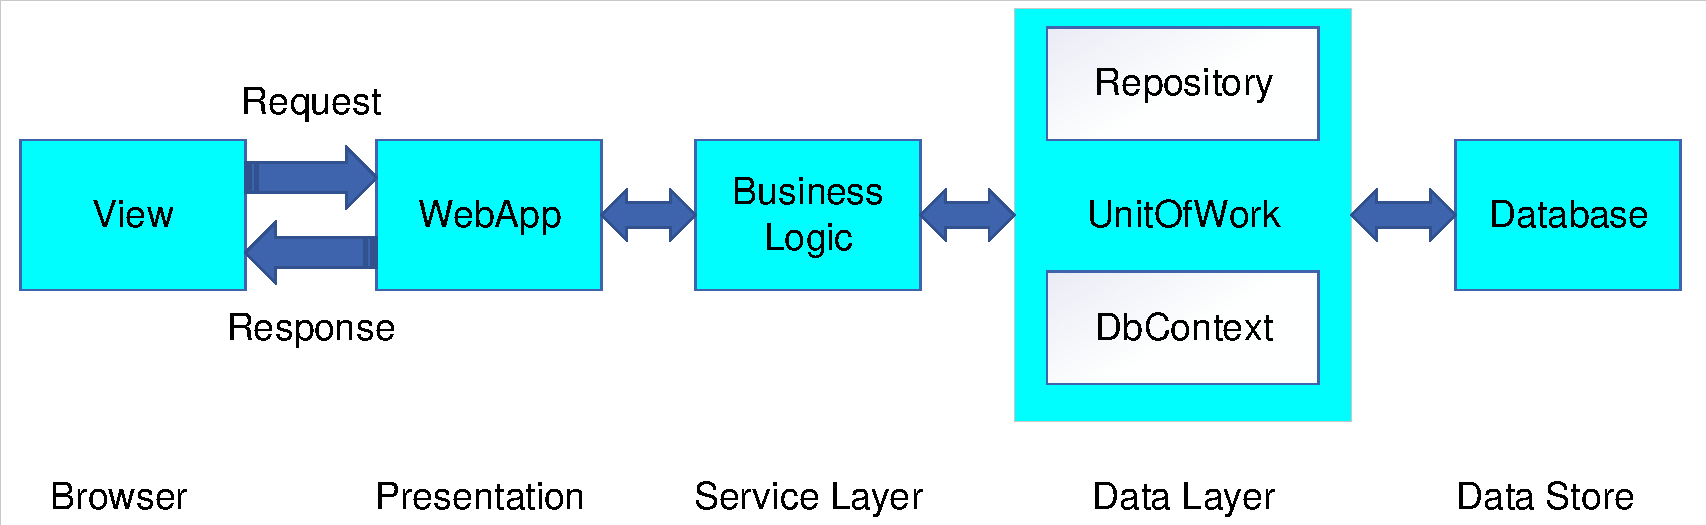
\includegraphics[scale=0.6]{image/MohinhDuongDiDuLieu.pdf}
    \end{center}
    \caption{Mô hình triển khai hệ thống}
    \label{refhinh4_1}
    \end{figure}
\end{center}

\par
Hình \ref{refhinh4_1} là mô hình tổng quan triển khai hệ thống bao gồm các tầng sau:
\begin{itemize}
\item Tầng View: tầng hiển thị giao diện cho người dùng.
\item Tầng WebApp: tầng tiếp nhận yêu cầu của người dùng để xử lý và trả dữ liệu đến view hiển thị lên giao diện người dùng, đây cũng là tầng trung gian giữa giao diện và dữ liệu nói cách khác WebApp là tầng điều khiển dữ liệu cho hệ thống.
\item Tầng Business Logic: tầng này xử lý các nghiệp vụ của từng thực thể có trong hệ thống như là sản phẩm, tài khoản, đơn hàng,...
\item Tầng Data Layer: tầng này đảm nhận việc điều khiển dữ liệu trong cơ sở dữ liệu thông qua Entity Framework, nó giúp hệ thống gọi đến cơ sở dữ liệu và thực hiện lấy đúng dữ liệu theo yêu cầu của người dùng.
\item Tầng Data Store: tầng này có nhiệm vụ lưu trữ dữ liệu cho hệ thống.
\end{itemize}
\par
Từ Hình \ref{refhinh4_1} em chia hệ thống thành 5 project theo như phân tầng đã trình bày ở trên. Đặt tên project của hệ thống là ShoppingOnline và mỗi project nhỏ sẽ được đặt tên theo quy tắc ShoppingOnline cộng với tên project nhỏ:
\begin{itemize}
\item ShoppingOnline.Infrastructure: Project này để hạng tầng chung của hệ thống.
\item ShoppingOnline.Utilities: Project này để khai báo các lớp tiện ích như: các hằng số, một số lớp mở rộng.
\item ShoppingOnline.Data: Project này để khai báo các thực thể có trong cơ sở dữ liệu.
\item ShoppingOnline.Data.EF: Project này gồm có: triển khai các repository, chứa DbContext  để thực hiện các truy vấn và kết nối đến cơ sở dữ liệu.
\item ShoppingOnline.Application: Project này triển khai các chức năng của mỗi thực thể có trong hệ thống.
\item ShoppignOnline.Application.Dapper: Project bao gồm một số chức năng mà Entity Framework không hỗ trợ nên phải dùng ngôn ngữ SQL thuần để truy vấn dữ liệu.
\item ShoppingOnline.WebApplication: Project được chạy lên đầu tiên khi bắt đầu hệ thống nó gồm có Controller để điểu khiển qua lại các yêu cầu từ View, một số tệp dùng để cài đặt Dependency Injection và cài đặt một số framework sử dụng thêm. 
\end{itemize}

\section{Kiểm thử hệ thống và kết quả}
\subsection{Kiểm thử}
- Kiểm thử chức năng đăng nhập:
\begin{longtable}[htp]{ |m{0.2\linewidth}|m{0.2\linewidth}|m{0.2\linewidth}|m{0.2\linewidth}|m{0.1\linewidth}|}
 \caption{Bảng kiểm thử chức năng đăng nhập \label{updateProduct}}\\
 \hline
Bước kiểm tra & Dữ liệu nhập vào & Kết quả dự kiến & Kết quả thực tế & Trạng thái \\
 \hline
Điều hướng đúng đến trang đăng nhập quản trị & &Người dùng đến được trang đăng nhập quản trị & Như dự kiến & Thành công\\
 \hline
 Nhập tên tài khoản & admin & Nhập được dữ liệu trên màn hình & Như dự kiến & Thành công\\
 \hline
  Nhập mật khẩu & 123654\$ & Nhập được dữ liệu trên màn hình & Như dự kiến & Thành công\\
 \hline
  Nhấn vào nút đăng nhập & & Người dùng được đăng nhập vào trang chủ quản trị & Như dự kiến & Thành công\\
 \hline
  Chuyển đến trang chủ quản trị & & Màn hình hiển thị thanh menu chức năng theo đúng quyền mà tài khoản được cấp & Như dự kiến & Thành công\\
 \hline
\end{longtable}

- Kiểm thử chức năng đăng xuất:
\begin{longtable}[htp]{ |m{0.2\linewidth}|m{0.2\linewidth}|m{0.2\linewidth}|m{0.2\linewidth}|m{0.1\linewidth}|}
 \caption{Bảng kiểm thử chức năng đăng xuất \label{updateProduct}}\\
 \hline
 Bước kiểm tra & Dữ liệu nhập vào & Kết quả dự kiến & Kết quả thực tế & Trạng thái \\
 \hline
  Nhấn vào nút đăng xuất & & Người dùng được chuyển về trang đăng xuất & Như dự kiến & Thành công\\
 \hline
\end{longtable}

- Kiểm thử chức năng quản lý tài khoản người dùng:
\begin{longtable}[htp]{ |m{0.2\linewidth}|m{0.2\linewidth}|m{0.2\linewidth}|m{0.2\linewidth}|m{0.1\linewidth}|}
 \caption{Bảng kiểm thử chức năng thêm tài khoản người dùng \label{updateProduct}}\\
 \hline
 Bước kiểm tra & Dữ liệu nhập vào & Kết quả dự kiến & Kết quả thực tế & Trạng thái \\
 \hline
  Nhấn vào nút thêm tài khoản người dùng & & Giao diện hiển thị modal nhập thông tin tài khoản & Như dự kiến & Thành công\\
 \hline
   Nhập tên đầy đủ & Lê Bá Tuấn Anh & Nhập được dữ liệu trên màn hình & Như dự kiến & Thành công\\
 \hline
   Nhập tên tài khoản & lebatuananh & Nhập được dữ liệu trên màn hình & Như dự kiến & Thành công\\
 \hline
   Nhập ngày sinh & 30/04/1996 & Nhập được dữ liệu trên màn hình & Như dự kiến & Thành công\\
 \hline
   Nhập mật khẩu & 123654 & Nhập được dữ liệu trên màn hình & Như dự kiến & Thành công\\
 \hline
   Nhập lại mật khẩu & 123654 & Nhập được dữ liệu trên màn hình & Như dự kiến & Thành công\\
 \hline
   Nhập email & tuananh300496 @gmail.com & Nhập được dữ liệu trên màn hình & Như dự kiến & Thành công\\
 \hline
   Nhập địa chỉ & Hà Nội & Nhập được dữ liệu trên màn hình & Như dự kiến & Thành công\\
 \hline
   Nhập số điện thoại & 0333355553 & Nhập được dữ liệu trên màn hình & Như dự kiến & Thành công\\
 \hline
   Chọn giới tính & Male & Nhập được dữ liệu trên màn hình & Như dự kiến & Thành công\\
 \hline
   Chọn nhóm quyền cho tài khoản & Top Manager & Nhập được dữ liệu trên màn hình & Như dự kiến & Thành công\\
 \hline
    Chọn trạng thái tài khoản & Active & Nhập được dữ liệu trên màn hình & Như dự kiến & Thành công\\
 \hline
    Nhấn nút lưu tài khoản && Hiển thị thông báo tài khoản được lưu và chuyển về trang danh sách tài khoản  & Như dự kiến & Thành công\\
 \hline
\end{longtable}

- Kiểm thử chức năng quản lý sản phẩm:
\begin{longtable}[htp]{ |m{0.2\linewidth}|m{0.2\linewidth}|m{0.2\linewidth}|m{0.2\linewidth}|m{0.1\linewidth}|}
 \caption{Bảng kiểm thử chức năng thêm sản phẩm \label{updateProduct}}\\
 \hline
 Bước kiểm tra & Dữ liệu nhập vào & Kết quả dự kiến & Kết quả thực tế & Trạng thái \\
 \hline
  Nhấn vào nút thêm sản phẩm & & Giao diện hiển thị modal nhập thông tin sản phẩm & Như dự kiến & Thành công\\
 \hline
   Nhập tên sản phẩm & Sản phẩm Test & Nhập được dữ liệu trên màn hình & Như dự kiến & Thành công\\
 \hline
   Chọn danh mục sản phẩm & Women shirt & Nhập được dữ liệu trên màn hình & Như dự kiến & Thành công\\
 \hline
   Nhập mô tả cho sản phẩm & Sản phẩm Test & Nhập được dữ liệu trên màn hình & Như dự kiến & Thành công\\
 \hline
   Nhập đơn vị & chiếc & Nhập được dữ liệu trên màn hình & Như dự kiến & Thành công\\
 \hline
   Nhập giá bán  & 10000 & Nhập được dữ liệu trên màn hình & Như dự kiến & Thành công\\
 \hline
   Nhập giá nhập & 5000 & Nhập được dữ liệu trên màn hình & Như dự kiến & Thành công\\
 \hline
   Nhập giá khuyến mại & 8000 & Nhập được dữ liệu trên màn hình & Như dự kiến & Thành công\\
 \hline
   Tải ảnh lên và chọn kích cỡ cho ảnh & 0333355553 & Tải được dữ liệu trên màn hình & Như dự kiến & Thành công\\
 \hline
   Soạn thảo nội dung cho sản phẩm & Sản phẩm Test & Nhập được dữ liệu trên màn hình & Như dự kiến & Thành công\\
 \hline
    Chọn trạng thái, sản phẩm hot, hiển thị trên trang chỉ sản phẩm & Active, Hot product, Show on home & Nhập được dữ liệu trên màn hình & Như dự kiến & Thành công\\
 \hline
    Nhấn nút lưu sản phẩm && Hiển thị thông báo sản phẩm được lưu và chuyển về trang danh sách sản phẩm  & Như dự kiến & Thành công\\
 \hline
\end{longtable}

\subsection{Kết quả}
Trên đây em trình bày kiểm thử một số chức năng chính của hệ thống vì trong lúc triển khai hệ thống em đã kiểm thử hết các chức năng của hệ thống và dưới đây là một số kết quả sau khi kiểm thử phần mềm.
 \begin{center}
    \begin{figure}[h]
    \begin{center}
     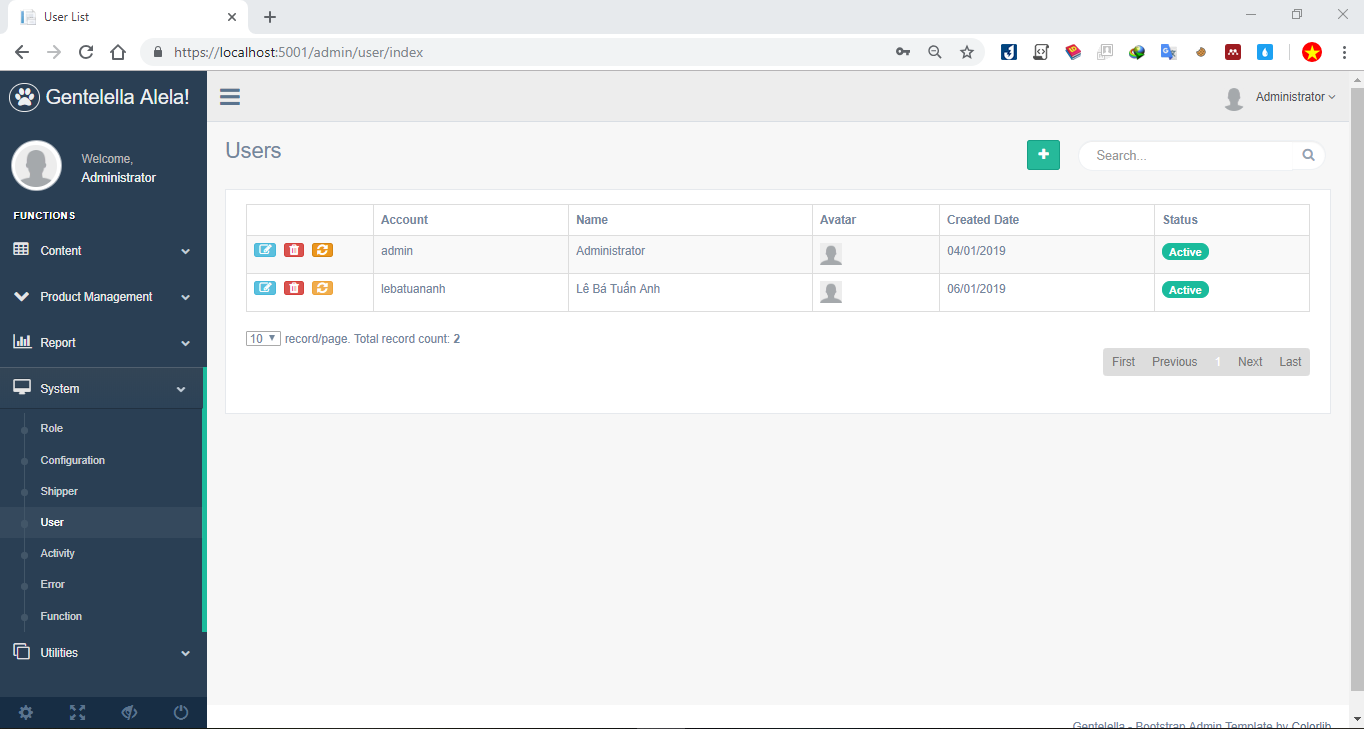
\includegraphics[scale=0.45]{image/danhsachTK}
    \end{center}
    \caption{Giao diện danh sách tài khoản}
    \label{refhinh4_2}
    \end{figure}
\end{center}
\par
Hình \ref{refhinh4_2} là màn hình sau khi kiểm thử chức năng thêm tài khoản người dùng. Một số hình dưới đây đều là kết quả thu được sau khi quá trình kiểm thử triển khai hệ thống, vì có nhiều chức năng nên em chỉ đưa ra những hình ảnh của chức năng nổi bật nhất.
 \begin{center}
    \begin{figure}[h]
    \begin{center}
     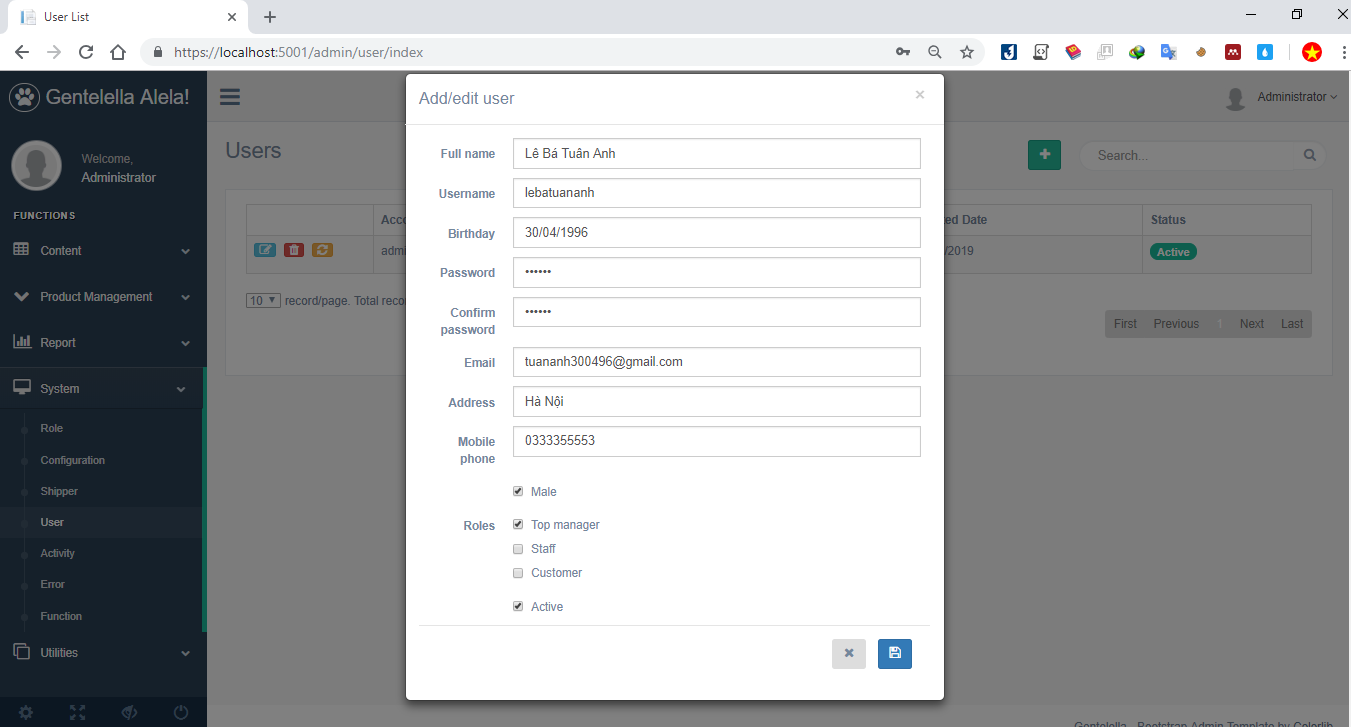
\includegraphics[scale=0.45]{image/themTK}
    \end{center}
    \caption{Giao diện thêm tài khoản}
    \label{refhinh4_3}
    \end{figure}
\end{center}

 \begin{center}
    \begin{figure}[h]
    \begin{center}
     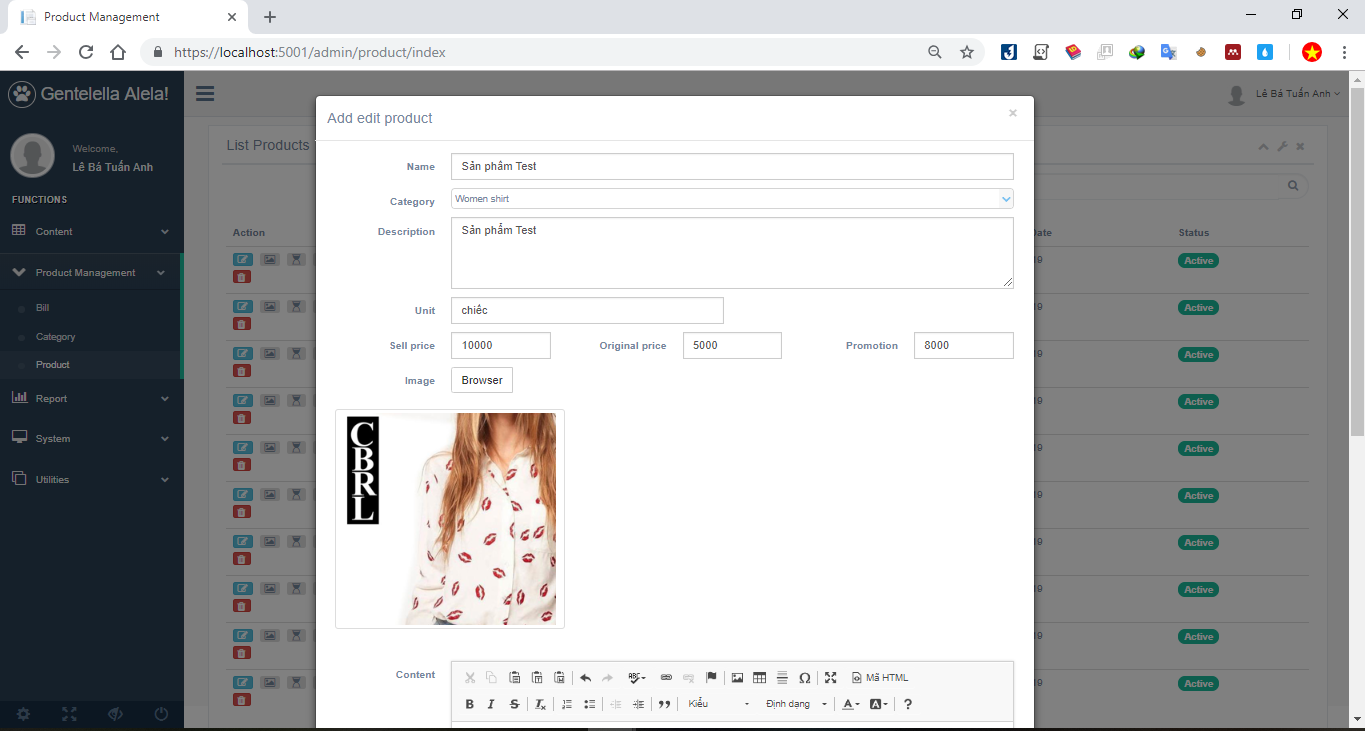
\includegraphics[scale=0.45]{image/themSanpham}
    \end{center}
    \caption{Giao diện thêm sản phẩm}
    \label{refhinh4_4}
    \end{figure}
\end{center}

\begin{center}
    \begin{figure}[h]
    \begin{center}
     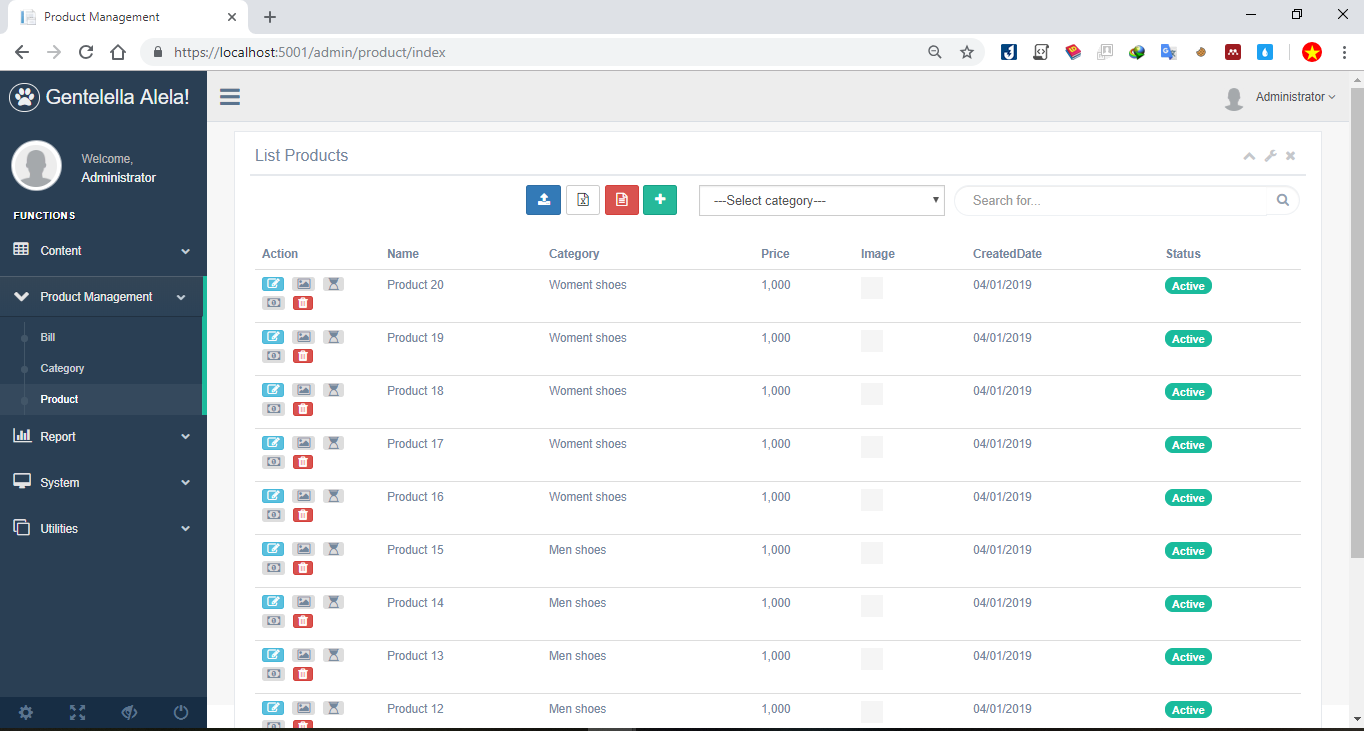
\includegraphics[scale=0.45]{image/danhsachSP}
    \end{center}
    \caption{Giao diện danh sách sản phẩm}
    \label{refhinh4_5}
    \end{figure}
\end{center}

\begin{center}
    \begin{figure}[h]
    \begin{center}
     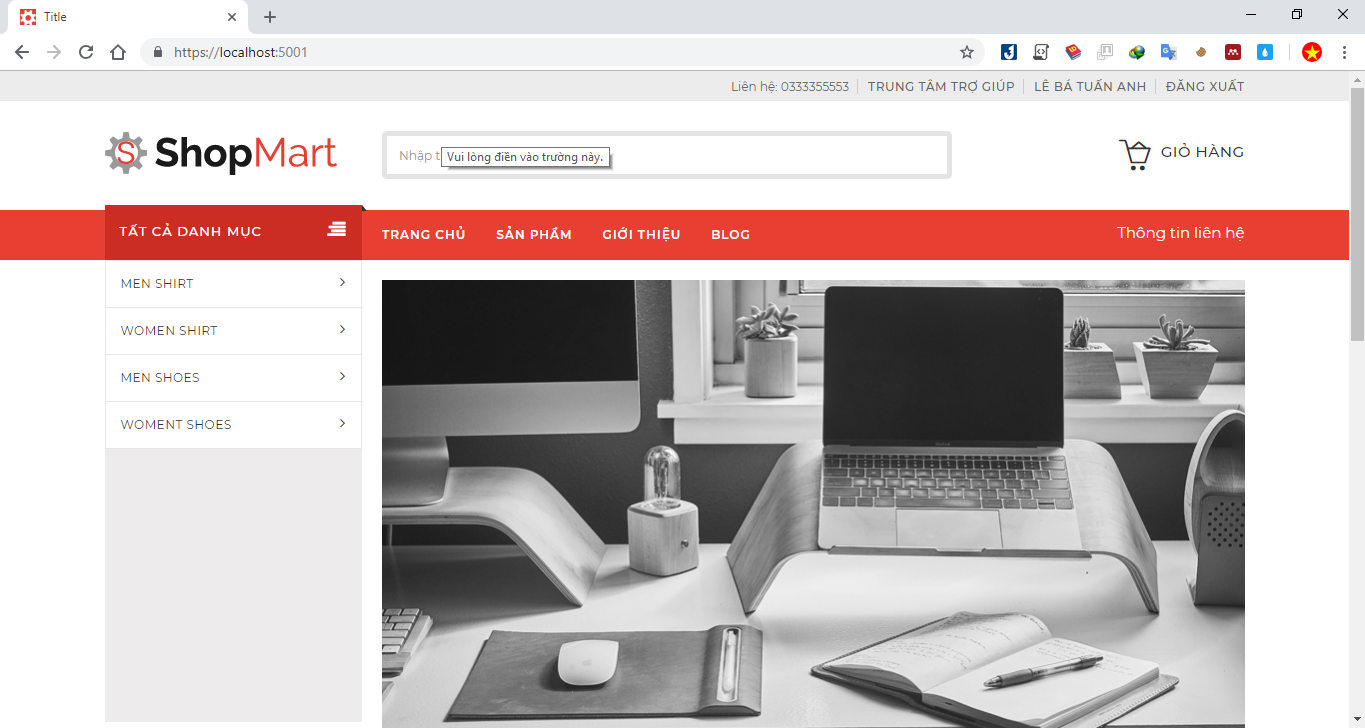
\includegraphics[scale=0.45]{image/trangchu}
    \end{center}
    \caption{Giao diện trang chủ}
    \label{refhinh4_6}
    \end{figure}
\end{center}




